\chapter{Proposed Methodology}
\noindent \rule{6.6in}{0.01in}
\vspace{0.5cm}

This chapter details the proposed Adaptive Predictive-Semantic Model (APSM) framework, which builds upon the decentralized Gossip Learning baseline to enable highly efficient workload forecasting. 

\section{System Model}
The system models a fully decentralized peer-to-peer edge computing network. We define the network as a graph $G = (V, E)$, where $V$ represents a set of resource-constrained edge computing nodes (e.g., edge servers, micro data centers, or IoT gateways), and $E$ represents the wireless or wired communication links between them. The network topology is constructed as a $k$-edge-connected graph, ensuring multiple distinct paths between any two nodes to guarantee fault tolerance against node or link failures.

Each edge node $i \in V$ is responsible for handling a continuous stream of incoming tasks or serverless functions. To proactively manage these tasks and prevent resource exhaustion, each node hosts a local Machine Learning (ML) model designed for univariate time-series forecasting. Specifically, the nodes utilize a Long Short-Term Memory (LSTM) neural network, a type of recurrent neural network exceptionally well-suited for capturing temporal dependencies in highly volatile workloads.

The nodes participate in the Gossip Learning (GL) protocol. The basic operational loop of a node in this system consists of three distinct phases:
\begin{enumerate}
    \item \textbf{Prediction:} The node utilizes its local LSTM model to predict the upcoming workload for the next time step.
    \item \textbf{Training:} Once the actual workload arrives, the node calculates the forecasting error and uses gradient descent (via backpropagation through time) to update the weights of its local LSTM model.
    \item \textbf{Gossiping:} The node selects a random neighbor from its local adjacency list and transmits its updated model. When a node receives a model from a neighbor, it mathematically merges the received weights with its own weights (typically using uniform averaging).
\end{enumerate}

\section{Problem Formulation and The APSM Filter}
While the baseline GL protocol blindly executes the Gossiping phase at every time step, the proposed APSM framework intervenes at this precise juncture. The core mathematical logic of APSM is to intercept the transmission and determine its semantic value before utilizing network bandwidth.

\subsection{Semantic Surprise Metric}
At any given discrete time step $t$, let $y(t)$ denote the actual incoming workload at an edge node, and let $\hat{y}(t)$ denote the workload predicted by the local LSTM model. The absolute prediction error, or the "surprise" metric $\epsilon(t)$, is defined as:
\begin{equation}
    \epsilon(t) = | y(t) - \hat{y}(t) |
\end{equation}
A high value of $\epsilon(t)$ indicates that the node encountered a workload pattern that it failed to predict accurately, implying that its current model lacks the necessary "knowledge" of this pattern. Conversely, a low $\epsilon(t)$ indicates that the node's model is already well-calibrated to the current traffic.

\subsection{Dynamic Adaptive Thresholding}
To determine what constitutes a "high" or "low" error, a static threshold cannot be used, as workload magnitudes fluctuate drastically throughout the day. Instead, APSM employs a dynamic, adaptive threshold based on the statistical variance of recent prediction errors.

Each node maintains a rolling window of its most recent prediction errors: $W = [\epsilon(t-w), \dots, \epsilon(t-1), \epsilon(t)]$, where $w$ is the window size (e.g., $w = 50$). 
The standard deviation of the errors in this window, $\sigma(\epsilon)$, is computed continuously. The adaptive threshold $\tau(t)$ is then mathematically formulated as:
\begin{equation}
    \tau(t) = K \times \sigma(\epsilon)
\end{equation}
Here, $K$ is a configurable sensitivity multiplier. Setting $K = 2.0$ approximates the 95\% confidence interval of a normal distribution. This ensures that the threshold automatically scales: during highly volatile periods, the threshold increases to prevent continuous triggering; during stable periods, the threshold tightens to capture subtle anomalies.

\subsection{The Semantic Suppression Rule}
Before transmitting its LSTM model to a neighbor, the edge node evaluates the Semantic Suppression Rule:
\begin{equation}
    \text{Action}(t) = 
    \begin{cases} 
      \text{Transmit Model}, & \text{if } \epsilon(t) > \tau(t) \\
      \text{Suppress Model}, & \text{if } \epsilon(t) \leq \tau(t)
    \end{cases}
\end{equation}

If the current prediction error $\epsilon(t)$ exceeds the dynamic threshold $\tau(t)$, the node has encountered a statistically significant "semantic surprise." Because the node has just trained its local model on this surprising data (in the Training phase), its model now contains valuable new knowledge that the rest of the network likely lacks. Therefore, the model is transmitted. 

If the error falls within the threshold boundaries, the node considers the local traffic pattern "predictable." Broadcasting a model trained on highly predictable, redundant data offers no mathematical benefit to neighboring nodes. The transmission is actively suppressed, instantly saving the energy required for wireless transmission and shielding the network from unnecessary congestion.

\vspace{1cm}
\begin{figure}[!ht]
    \centering
    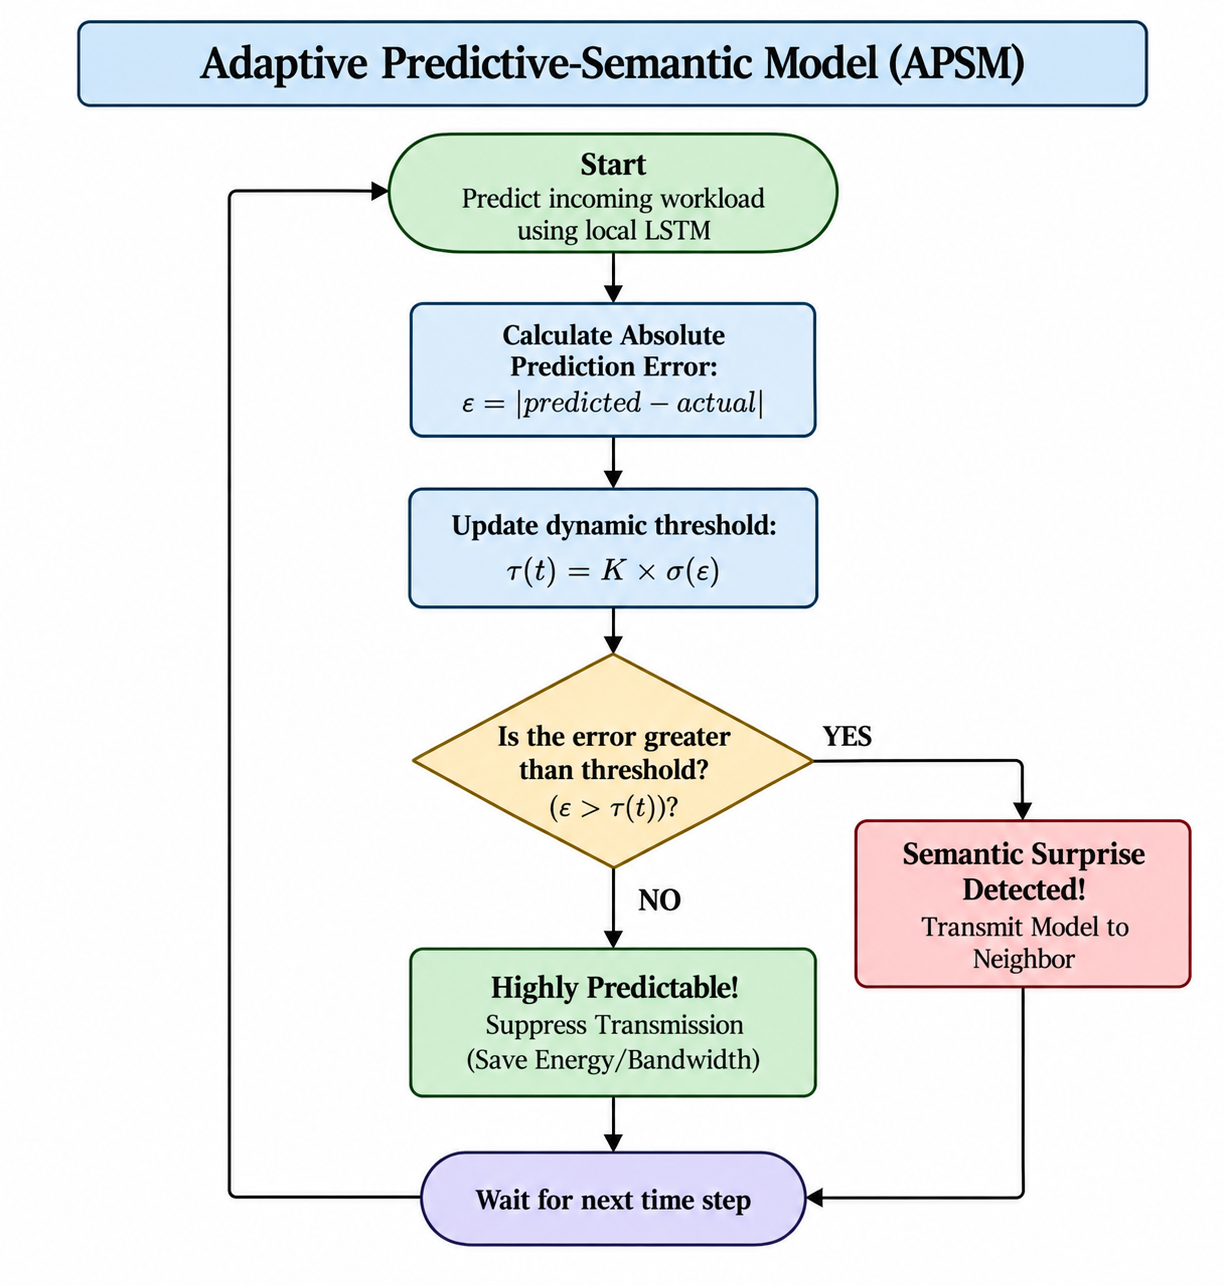
\includegraphics[width=0.6\textwidth]{chapters/figures/apsm_workflow.png}
    \caption{Flowchart of the Adaptive Predictive-Semantic Model (APSM) filtering logic.}
    \label{fig:apsm_flowchart}
\end{figure}
